\documentclass{beamer}

\usepackage[brazilian]{babel}
\usepackage[utf8]{inputenc}
\usepackage[T1]{fontenc}
\usepackage{xcolor}
\usepackage{listings}
\usepackage{color}
\usepackage{courier}
\usepackage{tikz}
\usepackage{verbatim}
\usepackage{cancel}

\definecolor{lightlightgray}{gray}{0.9}
\definecolor{OliveGreen}{cmyk}{0.64,0,0.95,0.40}
\definecolor{CadetBlue}{cmyk}{0.62,0.57,0.23,0}
\definecolor{codeback}{gray}{0.95}

\lstdefinestyle{CStyle}{
	basicstyle=\ttfamily,
	breakatwhitespace=false,
	breaklines=true,
	captionpos=b,
	keepspaces=true,
	numbers=left,
	numbersep=5pt,
	showspaces=false,
	showstringspaces=false,
	showtabs=false,
	tabsize=2,
	commentstyle=\color{OliveGreen},
	keywordstyle=\color{CadetBlue},
	language=C
}

\lstdefinestyle{customc}{
	belowcaptionskip=1\baselineskip,
	breaklines=true,
	%frame=L,
	tabsize=2,
	xleftmargin=\parindent,
	language=C,
	showstringspaces=false,
	%basicstyle=\scriptsize\ttfamily,
    basicstyle=\tiny\ttfamily,
	keywordstyle=\bfseries\color{green!40!black},
	commentstyle=\itshape\color{purple!40!black},
	identifierstyle=\color{blue},
	stringstyle=\color{orange},
	backgroundcolor = \color{codeback},
}

\title{Linguagem C}
\subtitle{Uma revisão com foco em sistemas embarcados}
\author{Marcelo Barros e Daniel Carvalho
{\tiny \url{https://github.com/marcelobarrosalmeida/mbedc}}}
\institute{UFU/FEELT}
\date{\today}

%\usetheme{Luebeck}

\begin{document}

\begin{frame}
\titlepage
\end{frame}

\begin{frame}
\frametitle{Sumário}
\tableofcontents
\end{frame}

\section{Introdução}
	
\begin{frame}
	\frametitle{Versões utilizadas}
	\begin{itemize}
		\item Versão C11 (ISO/IEC 9899:2011)
		\item Compilador GNU GCC\footnote{\url{https://www.onlinegdb.com/online_c_compiler}}
	\end{itemize}
\end{frame}

\begin{frame}
	\frametitle{Linha do tempo da linguagem C}
	\begin{description}
		\item[ B (1972):] Primeira implementação, Dennis Ritchie and Ken Thompson e colegas para o PDP11.
		\item [K\&R (1978):] Primeira especificação informal.
		\item [C89/C90 (1989/1990):] Adoção como padrão pela ANSI (C89) e depois pela ISO (C90).
		\item [C99 (1999):] Primeira grande revisão do padrão, amplamente utilizada.
		\item [C11 (2011):] Segunda revisão da linguagem. Aproximação ao C++. 
		\item [C17 (2018):] Sem características novas. Apenas correções.
		\item [C2x (2023?)]\footnote{\url{https://en.wikipedia.org/wiki/C2x}}
	\end{description}
\end{frame}

\begin{frame}
	\frametitle{Embedded C}
	{Existe uma linguagem ``Embedded C'' ?}
	\vspace*{0.5cm}
	\begin{itemize}
		\item Tecnicamente é apenas uma extensão do C, cobrindo:
	\begin{itemize}
		\item Aritmética de ponto fixo
		\item Espaço de endereçamento
		\item Endereçamento de hardware básico para I/O
	\end{itemize}
		\item Norma: \textit{Programming languages — C — Extensions to support embedded processors}
		ISO/IEC TR 18037:2008
	\end{itemize}
\end{frame}

\begin{frame}
	\frametitle{Palavras Reservadas}
	\begin{itemize}
	\item Não devem ser usadas como nomes de funções ou variáveis
	\item São \textit{case sensitive}
	\item Em azul, as adições do C11 em relação ao C99
\end{itemize}
\vspace*{0.5cm}
	\fbox{
	\begin{minipage}{10cm}
    {\small
		\texttt{auto break case char const continue default do double else enum extern float
		for goto if inline int long register restrict return short signed sizeof
		static struct switch typedef union unsigned void volatile while
		\_Bool \_Complex \_Imaginary}

		\texttt{\textcolor{blue}{\_Alignas \_Alignof \_Atomic  \_Generic
		\_Noreturn \_Static\_assert \_Thread\_local}}
        }
	\end{minipage}
	}
\end{frame}


\begin{frame}
	\frametitle{Estrutura e organização de uma aplicação}
	%\begin{center}
		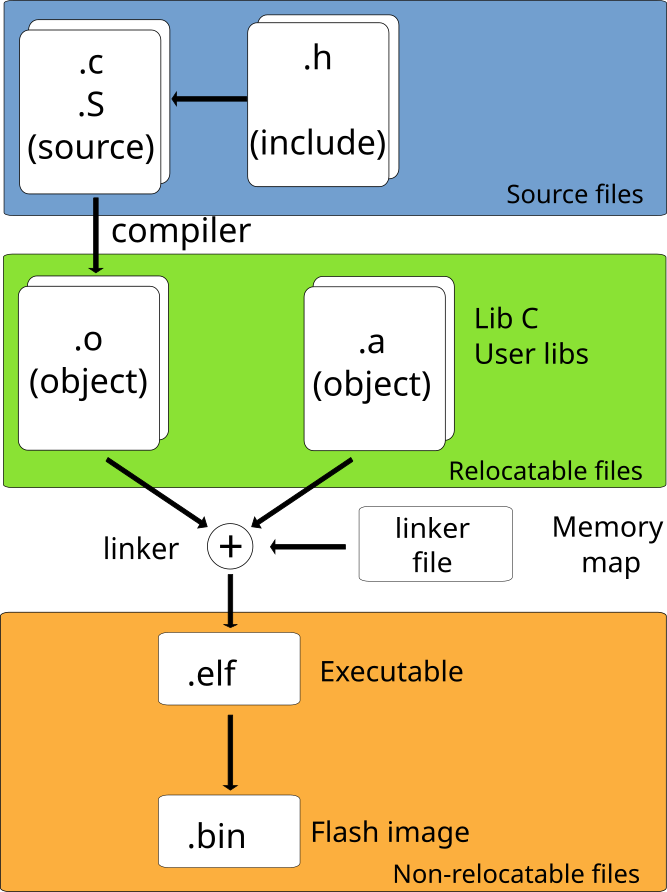
\includegraphics[scale=0.6]{imgs/compile_process.png}
	%\end{center}
\end{frame}

\section{Organização de arquivos de inclusão}
	
\begin{frame}
	\frametitle{Organização dos arquivos de inclusão}
	\begin{columns}[T] % align columns
		\begin{column}{.450\textwidth}
			\lstinputlisting[style=customc]{code/demo.h}
		\end{column}%
		\hfill%
		\begin{column}{.55\textwidth}
			\begin{itemize}
				\item Pense como API: só exporte interfaces e o que elas precisarem !
				\item Não esqueça a proteção de inclusão recursiva !
				\item Não é ANSI-C mas \texttt{\textcolor{blue}{\#pragma once}} pode ser interessante
				\item Não definir variáveis ou funções em .h
				\item Evite colocar arquivos de inclusão em .h (boa prática)
                \item E o \texttt{\textcolor{blue}{\_\_cplusplus}} e \texttt{\textcolor{blue}{extern ``C''}} ?
			\end{itemize}
		\end{column}%
	\end{columns}
\end{frame}

\begin{frame}[fragile]
	\frametitle{Name mangling ou name decoration}
		\begin{itemize}
			\item É uma forma de adicionar informações adicionais a nomes de funções, variáveis, etc, de forma a remover ambiguidade e gerar informação adicional ao linker\footnote{{\tiny\url{ https://bit.ly/3CuvCYe}}}.
			\item Por exemplo, como o compilador C++ irá gerar nomes únicos para uma função com \textit{overloading} ?
            	\begin{lstlisting}[style=customc]
void accel_read(float &x, float &y, float &x) {}
void accel_read(accel_t &data) {};
            	\end{lstlisting}
               \item Nomes decorados gerados pelo GCC (objdump -d <binário>):
            	\begin{lstlisting}[style=customc]
0000000000001149 <_Z9accel_readRfS_S_>:
0000000000001160 <_Z9accel_readR7accel_s>:
            	\end{lstlisting}
		\end{itemize}
\end{frame}

\begin{frame}[fragile]
	\frametitle{Name mangling ou name decoration}
		\begin{itemize}
			\item Logo, se você linkar um programa em C com outras partes em C++, o compilador C++ irá gerar um padrão de name decoration para as suas funções em C que é diferente dos símbolos gerados pelo C !
           \item A convenção de chamada padrão do C (\texttt{\textcolor{blue}{\_cdecl}})\footnote{\tiny{\url{https://en.wikipedia.org/wiki/Name_mangling}}} apenas adiciona ``\texttt{\textcolor{blue}{\_}}'' antes do nome das funções.
           \item Assim, se declarar a função como \texttt{\textcolor{blue}{extern ``C'' void func(void);}} você está explicitando que a decoração de \texttt{\textcolor{blue}{func}} deve seguir o padrão do C (\texttt{\textcolor{blue}{\_func}}).
           \item O \texttt{\textcolor{blue}{\_\_cplusplus}} é a forma de se identificar se é o compilador C++ quem está compilando o arquivo
		\end{itemize}
\end{frame}

\begin{frame}[fragile]
	\frametitle{E o extern ?}
	O externo permite explicitar a exportação do símbolo:
	\vspace*{0.5cm}
	\begin{description}
	\item [Para variáveis:] diz para o compilador que a variável citada existe em algum lugar, não aloca memória para ela. O linker vai cuidar de ``encontrar'' onde a declaração foi feita.
	\begin{verbatim}
extern uint8_t buffer[16];
	\end{verbatim}
	\item [Para funções:]	evidencia que a função tem linkagem externa, ou seja, o linker vai deixá-la disponível para ser ``encontrada'' por qualquer arquivo C. Esse é o default da linguagem. É o inverso do ``static''.
	\end{description}
		\vspace*{0.5cm}
		\begin{center}
		Atenção: \texttt{\textcolor{blue}{extern ``C'' <nome>}} é um dialeto C++ !
	\end{center}
\end{frame}

\begin{frame}
	\frametitle{Arquivos de inclusão (exemplo)}
	\lstinputlisting[style=customc]{code/accel.h}
\end{frame}

\section{Classes de armazenamento}

\begin{frame}
	\frametitle{Especificadores de classes de armazenamento}
	\begin{itemize}
	\item extern é uma das classes de armazenamento do C
	\item Existem outros especificadores !
	\item No entanto, precisamos entender antes como as variáveis são armazenadas e as seções de código !
	\end{itemize}
	\vspace*{0.5cm}
	\begin{center}
		\texttt{\textcolor{blue}{extern static auto register}}
	\end{center}
	
\end{frame}

\section{Seções de um programa}

\begin{frame}
	\frametitle{Seções de código e dados do programa para embarcados}
    Quando o programa é compilador, ele é dividido em \textbf{seções}:
    \vspace*{0.5cm}
    \begin{description}
    \item[text (flash):] Onde é armazenado o código executável de fato, geralmente em flash
    \item[rodata (flash):] Constantes do código (read only)
    \item[bss (RAM):] Local das variáveis que vão ser inicializadas com zero na partida (o usuário não fez uma inicialização de valor explícita)
    \item[data (RAM):] Locas das variáveis que tiveram valores iniciais definidos pelo usuário.
    \item[stack (RAM):] Parte da RAM usada para variável temporárias e passagem de parâmetros
    \item[heap (RAM):] Parte da RAM usada para alocações dinâmicas
    \end{description}
\end{frame}

\begin{frame}
	\frametitle{Exemplo de seções para um microcontrolador STM32F411}
	\begin{columns}[T] % align columns
	\begin{column}{.60\textwidth}
	\begin{itemize}
		\item Um arquivo de \textit{linkedição} (.ld) especifica as áreas de memória (flash e RAM) e como elas serão divididas para comportar as seções de text, bss, data, rodata, heap e stack.
        \item Um código de inicialização (que roda antes do \texttt{main()}) é responsável por preparar o terreno:
        	\begin{itemize}
        		\item Zerar a seção bss
                \item Inicializar a seção data
                \item Inicializar o ponteiro da pilha
                \item Inicializar o heap
        	\end{itemize}
	\end{itemize}
	\end{column}%
	\hfill%
	\begin{column}{.40\textwidth}
        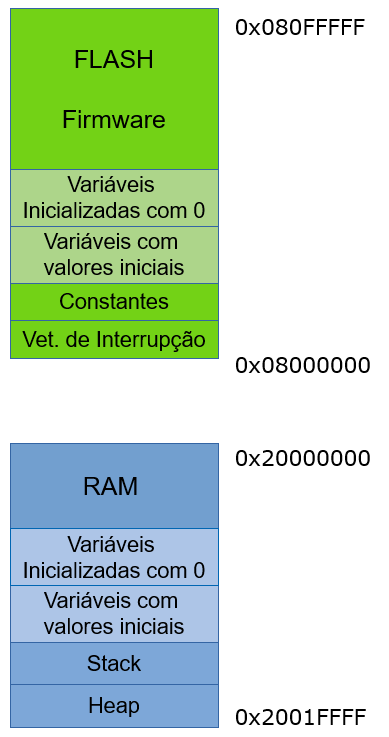
\includegraphics[scale=0.35]{imgs/sections.png}
	\end{column}%
\end{columns}
\end{frame}

\section{Uso da pilha}

\begin{frame}
	\frametitle{Stack (Pilha) e heap}
	\begin{itemize}
	\item Stack:
	\begin{itemize}
		\item Geralmente usado para alocação de variáveis temporárias ou passagem de parâmetros.
		\item É uma região linear de memória, normalmente gerida por um registro denominado de \textit{Stack Pointer}.
		\item O compilador analisa o código e gerar instruções para uso do stack.
	\end{itemize}
	\item Heap: uma área de memória reservada para as alocações dinâmicas de memória pelo programa (via chamadas como calloc/malloc)
	\end{itemize}
\end{frame}

\begin{frame}
	\frametitle{Stack (Exemplo)}
	\begin{columns}[T] % align columns
	\begin{column}{.55\textwidth}
		\lstinputlisting[style=customc]{code/stack.c}
	\end{column}%
	\hfill%
	\begin{column}{.45\textwidth}
    {\footnotesize
	\begin{itemize}
	\item \texttt{global\_sum}: na seção data
    \item \texttt{data}: temporariamente no stack
    \item \texttt{sum}: temporariamente no stack
    \item variáveis passadas na chamada da função \texttt{sum}: temporariamente no stack
    \item retorno do valor da função \texttt{sum}:temporariamente  no stack
	\end{itemize}
    }
	\end{column}%
\end{columns}
\end{frame}

\begin{frame}
	\frametitle{Cuidados no uso da pilha}
	\begin{itemize}
	\item Tamanho de variáveis e estouro de pilha
	\item Recursão ou longo encadeamento de chamadas
	\item Retorno de valores locais
	\item Dimensionamento da pilha
	\end{itemize}
\end{frame}

\begin{frame}
	\frametitle{Formas de dimensionamento da pilha}
	\begin{itemize}
		\item Análises estáticas
		\begin{itemize}
			\item Usando o próprio compilador (\texttt{-fstack-usage} e \texttt{-fcallgraph-info} no GCC) e analisando o uso da pilha a partir do \texttt{main()} (análise estática)
			\item Usando ferramentas (PC-Lint, valgrind, cppcheck)
			\item Problemas: podem falhar em casos de recursão, interrupções, chamadas indiretas (ponteiros para função)
		\end{itemize}
		\item Análises dinâmicas: técnica da marca d'agua na região do stack (verificação dinâmica, útil em caso de recursão, interrupção)
		\end{itemize}
\end{frame}

\begin{frame}
	\frametitle{Retomando: especificadores de classe de armazenamento}
		Uso de static em variáveis e funções:
	\vspace*{0.5cm}
	\begin{itemize}
	\item static em variáveis locais:
		\begin{itemize}
		\item Escopo local (não visível fora da função)
		\item Armazenamento em área global (não usa pilha)
		\item Permite valores de inicialização.
		\end{itemize}
	\item static em variáveis globais: linkagem interna para a variável (não ``visível'' por outros arquivos).  Isso permite, por exemplo, ter \textit{nomes de variáveis iguais em arquivos diferentes}.
	\item static em funções: linkagem interna para a função, similar a variáveis.
	\end{itemize}
\end{frame}

%\begin{frame}
%	\frametitle{Especificadores de classes de armazenamento}
%		\begin{center}
%		\texttt{\textcolor{blue}{static}}
%		\end{center}
%		\vspace*{0.5cm}
%		\begin{itemize}
%			\item Se usada com variáveis dentro de funções: gera variáveis que mantem valores entre chamadas e são alocadas na área de variáveis globais. São inicializadas com zero, caso não explicitamente especificado.
%			\item Se usada com variáveis no escopo do arquivo (fora das funções) o comportamento é o mesmo mas existem diferenças em relação a sua visibilidade.
%			\item \texttt{static} também pode ser usada em declarações de função. Novamente, implica em mudança de visibilidade.
%			\item Novo conceito requerido: \textbf{linkagem padrão da linguagem C} !
%		\end{itemize}
%\end{frame}

\begin{frame}
	\frametitle{Exemplo de static e variáveis locais}
	\begin{columns}[T] % align columns
		\begin{column}{.60\textwidth}
			\lstinputlisting[style=customc]{code/static_var_fun.c}
		\end{column}%
		\hfill%
		\begin{column}{.40\textwidth}
    {\footnotesize
	\begin{itemize}
	\item \texttt{initialized}: na seção de variáveis globais mas sem visibilidade fora de \texttt{drv\_init}, com valore inicial \texttt{false} e mantendo o valor entre chamadas da função
    \item \texttt{data}: idem, não penalizando o stack
	\end{itemize}
    }
		\end{column}%
	\end{columns}
\end{frame}

\begin{frame}
	\frametitle{Detalhes: retorno de valores locais, da pilha, pode ?}
	\begin{center}
	\lstinputlisting[style=customc]{code/stack_ret_a.c}
	\end{center}
	\pause
	\begin{tikzpicture}[remember picture, overlay]
		\node [xshift=-2cm,yshift=-4cm] at (current page.north east)	{
\includegraphics[scale=0.6]{imgs/ok.png}};
		\node [xshift=-2cm,yshift=-5.5cm] at (current page.north east)	{
\includegraphics[scale=0.6]{imgs/ok.png}};
		\node [xshift=-2cm,yshift=-7cm] at (current page.north east)	{
\includegraphics[scale=0.6]{imgs/maybe.png}};
	\end{tikzpicture}
\end{frame}

\begin{frame}
	\frametitle{Detalhes: retorno de valores locais, da pilha, pode ?}
	\begin{center}
		\lstinputlisting[style=customc]{code/stack_ret_b.c}
	\end{center}
	\pause
	\begin{tikzpicture}[remember picture, overlay]
		\node [xshift=-2cm,yshift=-4cm] at (current page.north east)	{
\includegraphics[scale=0.6]{imgs/maybe.png}};
		\node [xshift=-2cm,yshift=-5.5cm] at (current page.north east)	{
\includegraphics[scale=0.6]{imgs/nok.png}};
		\node [xshift=-2cm,yshift=-7cm] at (current page.north east)	{
\includegraphics[scale=0.6]{imgs/ok.png}};
\end{tikzpicture}
\end{frame}

\begin{frame}
	\frametitle{Especificadores de classes de armazenamento (auto)}
\begin{columns}[T] % align columns
	\begin{column}{.55\textwidth}
		\lstinputlisting[style=customc]{code/auto.c}
	\end{column}%
	\hfill%
	\begin{column}{.45\textwidth}
		\begin{center}
			\texttt{\textcolor{blue}{auto}}
		\end{center}
		\vspace*{0.5cm}
		\begin{itemize}
			\item É a classe padrão, de escopo local, armazenadas na RAM (pilha), valor inicial pode ser lixo.
			\item Pode ser omitida, por simplicidade.
		\end{itemize}
	\end{column}%
\end{columns}
\end{frame}

\begin{frame}
	\frametitle{Especificadores de classe de armazenamento (extern)}
	\begin{columns}[T] % align columns
		\begin{column}{.57\textwidth}
			\lstinputlisting[style=customc]{code/static_linkage_b.c}
			\lstinputlisting[style=customc]{code/static_linkage_a.c}
		\end{column}%
		\hfill%
		\begin{column}{.43\textwidth}
			\begin{itemize}
				\item Por default, o compilador C externa todos os símbolos gerados (main,var).
				\item Com \texttt{extern}, você pode explicitamente dizer que existe algo externo ao seu arquivo (file2.c) e que pretende usar.
			\item No entanto, mesmo que não especifique nada, o linker vai tentar encontrar algo na tabela de símbolos que resolva a referência.
			\end{itemize}
		\end{column}%
	\end{columns}
\end{frame}

\begin{frame}
	\frametitle{Especificadores de classe de armazenamento (static/extern)}
	\begin{columns}[T] % align columns
		\begin{column}{.57\textwidth}
			\lstinputlisting[style=customc]{code/static_linkage_e.c}
			\lstinputlisting[style=customc]{code/static_linkage_d.c}
			\lstinputlisting[style=customc]{code/static_linkage_c.c}
		\end{column}%
		\hfill%
		\begin{column}{.43\textwidth}
			\begin{itemize}
				\item Agora \texttt{var} tem \textbf{linkagem interna}, não é mais vista fora de file2.c (o símbolo não é exportado)
				\item Conceito também válido para funções \texttt{static} !
				\item Princípio de encapsulamento ou API.
			\end{itemize}
		\end{column}%
	\end{columns}
\end{frame}

\begin{frame}
	\frametitle{Especificadores de classe de armazenamento}
	\begin{center}
		\texttt{\textcolor{blue}{register}}
	\end{center}
	\vspace*{0.5cm}
	\begin{itemize}
		\item Se usada com variáveis dentro de funções.
		\item Indica ao compilador que deseja o armazenamento da variável em um registro do processador (geralmente para maior performance).
		\item Pouco útil atualmente, em geral o compilador resolve bem essas situações.
	\end{itemize}
\end{frame}

\section{Passagem por valor e referência}

\begin{frame}[fragile]
	\frametitle{Passagem por valor x passagem por referência}
	\begin{itemize}
		\item Passagem por valor: o valor original é copiado e não pode ser alterado pela função
		\item Passagem por referência:
		\begin{itemize}
			\item O valor original não é copiado e pode ser alterado pela função.
            \item É utilizado um ponteiro para essa operação, ou seja, deve ser passado o endereço do dado (referência) e não o seu valor.
			\item Também é interessante quando se passam estruturas muito grandes, economizando memória e processamento
		\end{itemize}
	\end{itemize}
    {\tiny
	\begin{lstlisting}[style=customc]
    // passagem por valor
    void func1(uint32_t v){ v = v + 5; }
    // passagem por referencia
    void func2(uint32_t *v){ *v = *v + 5; }

    int main(void)
    {
      uint32_t v = 10;
      func1(v); // v nao sera alterado
      func2(&v); // v sera alterado (15)
      return 0;
    }
	\end{lstlisting}
    }
%    É preciso falar um pouco mais sobre ponteiros !
\end{frame}

\section{Uso de ponteiros}

\begin{frame}[fragile]
	\frametitle{Ponteiros}
	\begin{itemize}
		\item Um ponteiro armazena endereço de memória e não um valor !
		\item São referências indiretas para outras variáveis ou funções
		\item São declarados com o emprego do asterisco \texttt{\textcolor{blue}{``*''}}
		\item Endereços de variáveis podem ser obtidos com o uso do operador \texttt{\textcolor{blue}{``\&''}}
		\item Declaração básica de uma variável ponteiro:
	\end{itemize}
    {\footnotesize
	\begin{verbatim}
        <tipo_de_dado> *variavel;
        uint8_t *pbuffer;
        struct accel_s *paccel;
	\end{verbatim}
    }
\end{frame}

\begin{frame}[fragile]
	\frametitle{Ponteiros para variáveis}
	\begin{columns}[T] % align columns
	\begin{column}{.50\textwidth}
		\lstinputlisting[style=customc]{code/ptr_a.c}
	\end{column}%
	\hfill%
	\begin{column}{.50\textwidth}
	 {\tiny
	\begin{verbatim}
              Memory (32 bits)
           +-------------------+
0x20000000 |      var (10)     |<---+
           +-------------------+    |
0x20000004 |        ...        |    |
           +-------------------+    |
0x20000008 | pvar (0x20000000) |----+
           +-------------------+
0x2000000C |                   |
           +-------------------+
0x20000010 |                   |
           +------------------+
	\end{verbatim}
}
	\end{column}%
\end{columns}
\end{frame}

\begin{frame}[fragile]
	\frametitle{Ponteiros para estruturas}
	\begin{columns}[T] % align columns
	\begin{column}{.75\textwidth}
		\lstinputlisting[style=customc]{code/ptr_b.c}
	\end{column}%
	\hfill%
	\begin{column}{.25\textwidth}
	\end{column}%
\end{columns}
\end{frame}

\begin{frame}[fragile]
	\frametitle{Ponteiros e vetores}
		\lstinputlisting[style=customc]{code/ptr_c.c}
	 {\scriptsize
	 	\begin{verbatim}
V     = 0x55D2EBB8F020
&V    = 0x55D2EBB8F020
&V[0] = 0x55D2EBB8F020
&V[1] = 0x55D2EBB8F024
&V[2] = 0x55D2EBB8F028
&V[2] = 0x55D2EBB8F02C
	\end{verbatim}
	}
\end{frame}

\begin{frame}[fragile]
	\frametitle{Ponteiros e arrays de caracteres}
		\lstinputlisting[style=customc]{code/ptr_e.c}
	 {\scriptsize
	 	\begin{verbatim}
STR1 = 0x7FFE326EC8E5   <== stack
STR2 = 0x5585446ED004   <== global
STR3 = 0x7FFE326EC8D0   <== stack
STR1    ab,2
STR2    ab,2
STR3[0] ab,2
STR3[1] 12,2
	\end{verbatim}
	}
\end{frame}

\begin{frame}
	\frametitle{Aritmética de ponteiros}
	\textbf{Regra básica}: ao incrementar/decrementar um ponteiro, o valor adicionado/subtraído é igual ao tamanho do tipo de dado para o qual ele aponta.
	\lstinputlisting[style=customc]{code/ptr_d.c}
\end{frame}

\begin{frame}[fragile]
	\frametitle{Aritmética de ponteiros}
	\begin{columns}[T] % align columns
	\begin{column}{.4\textwidth}
	 {\footnotesize
	\begin{verbatim}




SIZE    = 8
TRANS   = 0x7FFD8F7F0DA0
PTRANS  = 0x7FFD8F7F0DA0
&PTRANS = 0x7FFD8F7F0D98
TRAN[0] = 0x7FFD8F7F0DA0
TRAN[1] = 0x7FFD8F7F0DA8
	\end{verbatim}
}
	\end{column}%
	\hfill%
	\begin{column}{.6\textwidth}
	 {\scriptsize
	\begin{verbatim}
                 Memory (64 bits)
               +-------------------+
0x7FFD8F7F0D98 |  0x7FFD8F7F0DA0   |---+
               +-------------------+   |
               |        ...        |   |
               +-------------------+   |
0x7FFD8F7F0DA0 |      TRANS[0]     |<--+
               +-------------------+
0x7FFD8F7F0DA8 |      TRANS[1]     |
               +-------------------+
0x7FFD8F7F0DB0 |      TRANS[2]     |
               +-------------------+
0x7FFD8F7F0DB8 |      TRANS[3]     |
               +-------------------+
	\end{verbatim}
}
	\end{column}%
\end{columns}
\end{frame}

\begin{frame}
	\frametitle{Ponteiros para função}
	\begin{itemize}
		\item O nome da função é um sempre um ponteiro !
		\item O grande problema é a notação, que é confusa !
	\end{itemize}
	\lstinputlisting[style=customc]{code/ptr_fun_a.c}
\end{frame}

\begin{frame}
	\frametitle{Ponteiros para função}
	\begin{itemize}
		\item Mas não precisa ser confuso assim ! O uso de typedef pode ajudar.
		\item Acompanhe como criar um ponteiro pra função e como o programa se transforma depois disso.
	\end{itemize}
	\vspace*{0.5cm}
    {\scriptsize
\texttt{int64\_t sum(int32\_t a, int32\_t b);} \\
\texttt{\textcolor{blue}{\textbf{typedef}}} \texttt{int64\_t sum(int32\_t a, int32\_t b);} \\
\texttt{\textcolor{blue}{typedef}} \texttt{int64\_t \texttt{\textcolor{blue}{\textbf{(}}}sum\texttt{\textcolor{blue}{\textbf{)}}}(int32\_t a, int32\_t b);} \\
\texttt{\textcolor{blue}{typedef}} \texttt{int64\_t \texttt{\textcolor{blue}{(\textbf{sum\_t})}}(int32\_t a, int32\_t b);} \\
\texttt{\textcolor{blue}{typedef}} \texttt{int64\_t \texttt{\textcolor{blue}{(\textbf{*}sum\_t)}}(int32\_t a, int32\_t b);} \\
\vspace*{0.5cm}
\texttt{typedef <retorno> (*nome\_do\_tipo)(lista,de,parâmetros);}
}
\end{frame}

\begin{frame}
	\frametitle{Ponteiros para função}
	\begin{itemize}
		\item Bem mais legível:
	\end{itemize}
	\lstinputlisting[style=customc]{code/ptr_fun_b.c}
\end{frame}

\begin{frame}
	\frametitle{Ponteiros para função (Exemplo completo)}
	\lstinputlisting[style=customc]{code/ptr_fun_c.c}
\end{frame}

\section{Qualificadores const e volatile}

\begin{frame}
	\frametitle{Qualificadores}
	\begin{center}
		\texttt{\textcolor{blue}{const volatile}}
	\end{center}
		\vspace*{0.5cm}
	\begin{description}
	\item [const:] indica que a variável é constante, ou seja, que seu valor não muda durante a execução. O compilador pode usar essa informação para colocar essa variável em flash e encontrar erros em tempo de compilação.
	\item [volatile:] indica que o valor da variável pode ser alterado por outros elementos além do fluxo de programa principal em execução. Exemplos:
    {\footnotesize
    \begin{itemize}
    \item Uma variável global compartilhada entre duas tarefas ou entre o programa principal e uma interrupção associadas a uma opção de compilação com maior nível de otimização.
    \item Uma variável que aponta para um registro do processador, ou seja, que pode ter o valor modificado pelo próprio hardware.
    \end{itemize}
    }
	\end{description}
\end{frame}

\begin{frame}
	\frametitle{Volatile}
	\begin{center}
		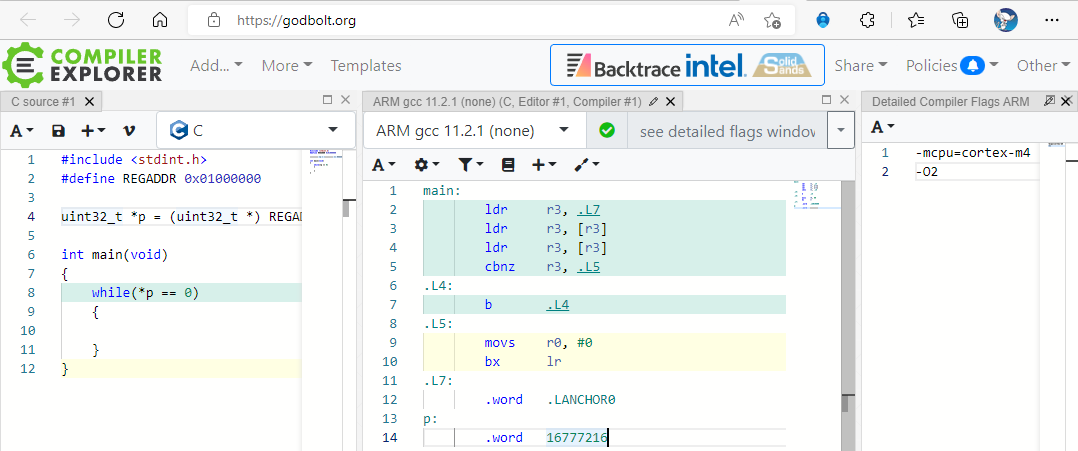
\includegraphics[scale=0.35]{imgs/vol1.png} \\
		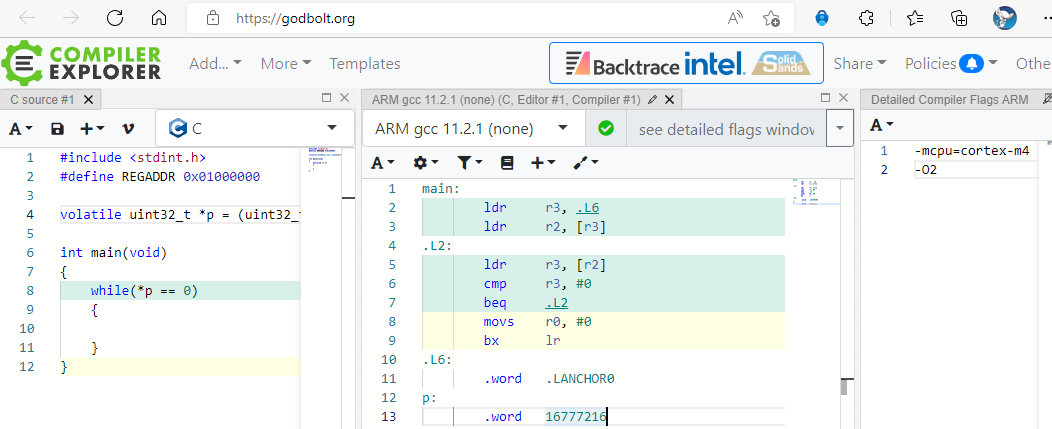
\includegraphics[scale=0.35]{imgs/vol2.png}
	\end{center}
\end{frame}

	
\begin{frame}[fragile]
	\frametitle{Qualificadores e ponteiros}
    Usar adequadamente o qualificador \texttt{const} com ponteiros é, frequentemente, uma boa prática:
		\vspace*{0.5cm}
	\begin{lstlisting}[style=customc]
void lcd_write(const uint8_t *data)
{
  // o dado apontado deve ser constante,
  // a linha abaixo gera um erro de compilacao
  data[0] = 1; // error: assignment of read-only location
}

void lcd_write(uint8_t *const data)
{
  // o ponteiro dever ser constante,
  // a linha abaixo gera um erro de compilacao
  data++; // error: increment of read-only parameter
}

void lcd_write(const uint8_t *const data)
{
  // o ponteiro dever ser constante,
  // assim como o dado apontado por ele !
}
	\end{lstlisting}
\end{frame}

\section{Enumerações, estruturas e uniões}

\begin{frame}[fragile]
	\frametitle{Estruturas}
	\begin{itemize}
	\item Ajudam a organizar os dados, evitando variáveis espalhadas.
	\item Melhoram a visualização e entendimento do código (legibilidade e manutenção).
	\item Reduzem complexidade, se bem usadas.
	\item \texttt{\textcolor{blue}{typedef}} pode ajudar !
	\end{itemize}
	\begin{columns}[T] % align columns
		\begin{column}{.5\textwidth}
	\begin{lstlisting}[style=customc]
struct coord_s
{
	uint32_t x;
	uint32_t y;
};

struct rect_s
{
  struct coord_s c1;
  struct coord_s c2;
};

struct rect_s rect = { 0 };
void func(struct rect_s *rect);
	\end{lstlisting}
		\end{column}%
		\hfill%
		\begin{column}{.5\textwidth}
	\begin{lstlisting}[style=customc]
typedef struct coord_s
{
	uint32_t x;
	uint32_t y;
} coord_t;

typedef struct rect_s
{
  coord_t c1;
  coord_t c2;
} rect_t;

rect_t rect = { 0 };
void func(rect_t *rect);
	\end{lstlisting}
		\end{column}%
	\end{columns}
\end{frame}

\begin{frame}[fragile]
	\frametitle{Enumerações}
	\begin{itemize}
	\item Permitem organizar definições relacionadas.
	\item Pode ajudar na detecção de erros (valores inválidos).
	\item Reduzem complexidade, melhoram a legibilidade.
	\item Obedecem regras de escopo, algo que não é possível com defines.
	\end{itemize}
	\begin{columns}[T] % align columns
		\begin{column}{.5\textwidth}
	\begin{lstlisting}[style=customc]
#define RTC_WEEKDAY_SUN 0
#define RTC_WEEKDAY_MON 1
#define RTC_WEEKDAY_TUE 2
#define RTC_WEEKDAY_WED 3
#define RTC_WEEKDAY_THU 4
#define RTC_WEEKDAY_FRI 5
#define RTC_WEEKDAY_SAT 6

void rtc_wday_set(uint8_t wday)
{
}
	\end{lstlisting}
		\end{column}%
		\hfill%
		\begin{column}{.5\textwidth}
	\begin{lstlisting}[style=customc]
typedef enum rtc_wday_e
{
  RTC_WEEKDAY_SUN = 0,
  RTC_WEEKDAY_MON = 1,
  RTC_WEEKDAY_TUE = 2,
  RTC_WEEKDAY_WED = 3,
  RTC_WEEKDAY_THU = 4,
  RTC_WEEKDAY_FRI = 5,
  RTC_WEEKDAY_SAT = 6,
} rtc_wday_t;

void rtc_wday_set(rtc_wday_t wday)
{
}
	\end{lstlisting}
		\end{column}%
	\end{columns}
\end{frame}

\begin{frame}[fragile]
	\frametitle{Uniões}
	\begin{itemize}
	\item Enquanto as estruturas dispõem sequencialmente os seus membros na memória, as uniões os armazenam na mesma posição.
	\item Isso permite ``visualizar'' a mesma área de memória com diferentes lentes.
	\item Em geral, muito útil em generalizações, evitando duplicações de memória.
	\end{itemize}
	\begin{columns}[T] % align columns
		\begin{column}{.5\textwidth}
	\begin{lstlisting}[style=customc]
typedef union kved_value_u
{
  uint8_t u8;
  uint16_t u16;
  uint32_t u32;
} kved_value_t;

typedef struct kved_data_s
{
  kved_value_t value;
  bool updated;
} kved_data_t;
	\end{lstlisting}
		\end{column}%
		\hfill%
		\begin{column}{.5\textwidth}
        {\tiny
	\begin{verbatim}
              Memory (32 bits)
           [________u32________] <- value.u32
           [___u16___]           <- value.u16
           [_u8]                 <- value.u8
           +---------+---------+
0x20000000 |    |    |    |    |
           +---------+---------+
0x20000004 |                   |
           +-------------------+
0x20000008 |        ...        |
           +-------------------+
	\end{verbatim}
    }
		\end{column}%
	\end{columns}
\end{frame}

\begin{frame}
	\frametitle{Exemplo completo (1/2)}
	\begin{columns}[T] % align columns
		\begin{column}{.5\textwidth}
		\lstinputlisting[style=customc]{code/struct_a.c}
			\end{column}%
		\hfill%
		\begin{column}{.5\textwidth}
		\lstinputlisting[style=customc]{code/struct_b.c}
		\end{column}%
	\end{columns}
\end{frame}

\begin{frame}
	\frametitle{Exemplo completo (2/2)}
	\begin{columns}[T] % align columns
		\begin{column}{.5\textwidth}
		\lstinputlisting[style=customc]{code/struct_c.c}
			\end{column}%
		\hfill%
		\begin{column}{.5\textwidth}
		\lstinputlisting[style=customc]{code/struct_d.c}
		\end{column}%
	\end{columns}
\end{frame}

\section{Organização de arquivos fonte}

\begin{frame}
	\frametitle{Arquivos de código fonte (modelo)}
	\begin{columns}[T] % align columns
		\begin{column}{.60\textwidth}
			\lstinputlisting[style=customc]{code/demo.c}
		\end{column}%
		\hfill%
		\begin{column}{.40\textwidth}
			\begin{itemize}
				\item Externe via funções o acesso a seus dados internos (encapsulamento)
				\item Dê escopo de arquivo para as suas funções e variáveis com \texttt{static} !
				\item Salve RAM colocando como \texttt{const} o que for realmente constante.
			\end{itemize}
		\end{column}%
	\end{columns}
\end{frame}

\begin{frame}
	\frametitle{Arquivos de códigos fonte (Exemplo)}
	\lstinputlisting[style=customc]{code/accel.c}
\end{frame}




\end{document}
